\documentclass[11pt,aspectratio=169]{beamer}

% -------------------- THEME & LAYOUT --------------------
\usetheme{Madrid}
\usecolortheme{dolphin} % base color scheme
\usefonttheme{professionalfonts}
\setbeamercovered{transparent}
\setbeamertemplate{navigation symbols}{}   % remove navigation buttons
\setbeamertemplate{caption}[numbered]      % numbered captions
\setbeamertemplate{itemize items}[triangle]
\setbeamersize{text margin left=1.2cm,text margin right=1.2cm} % adjust to taste

% -------------------- GLOBAL FONT SETTINGS --------------------

% 1. Force the base beamer font to small
\setbeamerfont{normal text}{size=\small}

% 2. Force math environments to follow the "small" font size
\setbeamerfont{math text}{size=\small}
\setbeamerfont{equation}{size=\small}

% 3. Redefine \normalsize itself 
% This ensures equations and lists (which look for \normalsize) use  instead.
\let\oldnormalsize\normalsize
\renewcommand{\normalsize}{\oldnormalsize\small}

% 4. Ensure lists also stay small
\setbeamerfont{itemize/enumerate body}{size=\small}
\setbeamerfont{itemize/enumerate subbody}{size=\small}

% -------------------- FONTS & TYPOGRAPHY --------------------
\usepackage[T1]{fontenc}
\usepackage[utf8]{inputenc}
\usepackage{newpxtext,newpxmath} % Palatino-like font & math
\usepackage{microtype}

% -------------------- MATH, TABLES & GRAPHICS --------------------
\usepackage{amsmath,amssymb,amsfonts,mathtools}
\usepackage{bm,booktabs,siunitx,graphicx}
\graphicspath{{./}{./figures/}}
%\numberwithin{equation}{section} % for numbered equations
% start counting at 4.0 so the first tag we use becomes 4.1
\setcounter{equation}{0}
\renewcommand{\theequation}{4.\arabic{equation}}

% -------------------- UTILITIES --------------------
\usepackage{appendixnumberbeamer}
\usepackage{ragged2e}
\usepackage{xspace}
\usepackage{csquotes}
\usepackage{xcolor}

% -------------------- HYPERREF --------------------
\hypersetup{
  colorlinks=false,
  pdfauthor={Francesca},
  pdftitle={Chapter 1 — The Value of Currency}
}

% -------------------- COLORS & EMPHASIS --------------------
\definecolor{myblue}{RGB}{0,70,140}
\definecolor{myred}{RGB}{180,30,30}
\definecolor{mygreen}{RGB}{0,120,70}
\definecolor{gold}{RGB}{184,134,11}

\setbeamercolor{title}{fg=gold}       % title page
\setbeamercolor{frametitle}{fg=gold}  % slide titles
\setbeamercolor{structure}{fg=gold}   % bullets, sections, links
\setbeamercolor{section in head/foot}{fg=gold,bg=black!10} % gold text on light background

% -------------------- FOOTLINE --------------------
\setbeamertemplate{footline}{
  \leavevmode%
  \hbox{%
    % Section links (hidden if no current section)
    \begin{beamercolorbox}[wd=0.7\paperwidth,ht=2.5ex,dp=1.5ex,leftskip=1.4em]{section in head/foot}%
      \ifx\insertsection\empty
        % nothing
      \else
        Section: \insertsection
      \fi
    \end{beamercolorbox}%
    % Frame number right
    \begin{beamercolorbox}[wd=0.3\paperwidth,ht=2.5ex,dp=1.5ex,leftskip=3.8cm]{section in head/foot}%
      \insertframenumber/\inserttotalframenumber
    \end{beamercolorbox}%
  }%
  \vskip1pt%
}

\newcommand{\highlight}[1]{\textcolor{myblue}{#1}}
\newcommand{\warning}[1]{\textcolor{myred}{#1}}

% -------------------- SHORTCUTS --------------------
\newcommand{\E}{\mathbb{E}}
\newcommand{\R}{\mathbb{R}}
\newcommand{\dd}{\mathrm{d}}
\newcommand{\mc}[1]{\mathcal{#1}}
\newcommand{\bb}[1]{\mathbb{#1}}
\newcommand{\uc}{U_c}
\newcommand{\zg}{Z_g}

% -------------------- TIGHTER DISPLAY MATH --------------------
\makeatletter
\g@addto@macro\normalsize{%
  \setlength\abovedisplayskip{8pt}%
  \setlength\belowdisplayskip{8pt}%
  \setlength\abovedisplayshortskip{6pt}%
  \setlength\belowdisplayshortskip{6pt}%
}
\makeatother
\setbeamertemplate{frametitle}{
  \nointerlineskip
  \begin{beamercolorbox}[wd=\paperwidth,ht=3.5ex,dp=1ex,center]{frametitle}
    \centering\insertframetitle
  \end{beamercolorbox}
}

% -------------------- METADATA --------------------
\title[Part I — Currency and Money]{\textbf{Part I: Currency and Money}\\[2pt]\large Chapter 4 — Private Money}
\author{Severin Rothen}
\institute{}
\date{\today}

% -------------------- SECTION ROADMAP --------------------
\AtBeginSection[]
{
  \begin{frame}
    \tableofcontents[currentsection, hideothersubsections]
  \end{frame}
}

% -------------------- Bibliography --------------------
\usepackage[backend=biber,style=authoryear]{biblatex}
\addbibresource{sources.bib}

\begin{document}

% ===================== TITLE SLIDE =====================
\begin{frame}[plain] % 'plain' removes header/footer for the title slide

\begin{columns}[T,totalwidth=\textwidth]

% ----- Left column: Main title, professor, chapter -----
\begin{column}{0.45\textwidth}
\vspace{2cm}

% Main title
{\usebeamercolor[fg]{title}\LARGE\textbf{Monetary Economics}\\[0.3cm]
\LARGE\textbf{and Policy}} 

\vspace{0.5cm}

% Professor name and date
{\large\textit{Pierpaolo Benigno}}\\[0.1cm]

\vspace{1cm}

% Chapter and subtitle
{\usebeamercolor[fg]{frametitle}\large Chapter 4: Private Money}

\end{column}

% ----- Right column: Image -----
\begin{column}{0.55\textwidth}
\vspace{1cm}
\centering
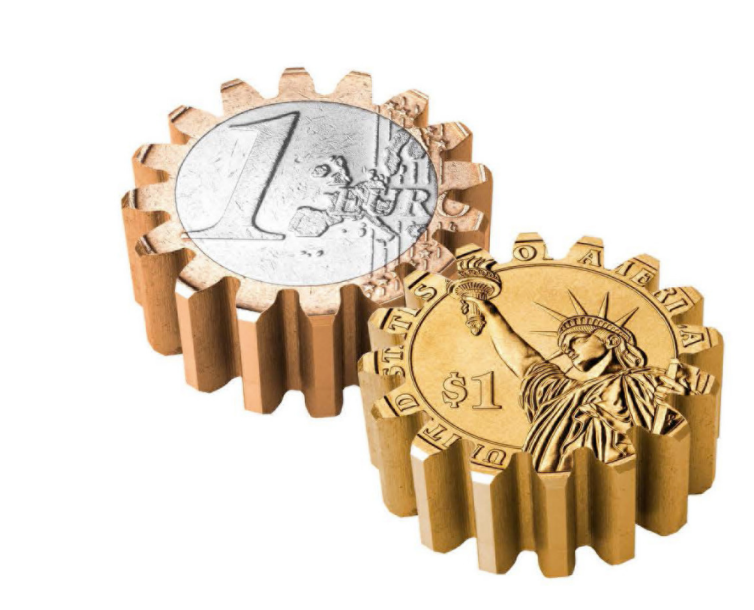
\includegraphics[width=0.9\linewidth]{Cover.png}
\end{column}

\end{columns}

% ----- Footer text (bottom-right corner) -----
\vspace*{2cm} % adjust if needed
\hfill{\large\textit{Prepared by Severin Rothen}}

\end{frame}

% 
\begin{frame}{What We Will Learn}
\small
\begin{itemize}

  \item How private intermediaries create \textbf{safe, money-like assets} and how these coexist with government-issued liquidity.

  \vspace{0.6em}

  \item Why private money creation does \emph{not} undermine the central bank’s \textbf{control of the price level}, thanks to interest on reserves and the backing principle.

  \vspace{0.6em}

  \item How competition eliminates liquidity premia, driving the economy toward \textbf{liquidity satiation} and zero rents.

  \vspace{0.6em}

  \item Under which conditions different institutional regimes  
  (free banking, narrow banking, real-bills–type arrangements)  
  yield \textbf{equivalent efficient allocations}.

  \vspace{0.6em}

  \item Why, in a multi-currency environment, the currency with \textbf{stable prices} becomes the dominant unit of account for safe assets, and how this affects welfare.
  
\end{itemize}
\end{frame}
% OUTLINE
\begin{frame}{Outline}
\tableofcontents
\end{frame}
%--------------------------------------------------
\section{Introduction}
\begin{frame}{Introduction}
\small
\begin{itemize}

  \item \textbf{Money vs.\ Currency}: Money is a claim on currency that shares similar \emph{properties} (store of value, medium of exchange).  
  Currency is money, but money is not necessarily currency.

  \vspace{0.6em}

  \item Government liabilities (cash, reserves, default-free bonds) are natural providers of liquidity, but \textbf{private intermediaries} can also create \emph{money claims} such as deposits.

  \vspace{0.6em}

  \item Classic insight from \textcite{Brunner1989HighPowered}:  
  financial intermediation creates a wedge between the \emph{monetary base} and the \emph{money stock}, because private claims also provide liquidity services.

\end{itemize}
\end{frame}

\begin{frame}{Introduction}
\small
\begin{itemize}

  \item By paying \emph{interest on reserves}, the central bank can separate the achievement of the inflation target from the efficient supply of  liquidity.

  \vspace{0.6em}

  \item \textbf{Backing principle}: price-level determination requires a real anchor, either through
  \begin{itemize}
    \item high-quality assets on the central bank’s balance sheet, or
    \item fiscal backing (taxation) supported by treasury--central bank cooperation.
  \end{itemize}

  \vspace{0.6em}

  \item The same logic applies to \textbf{liquidity supply}: abundant liquidity requires sufficient backing.

  \vspace{0.6em}

  \item Insufficient backing (few high-quality assets or weak fiscal capacity) can generate inefficiencies and instability.

  \vspace{0.6em}

  \item The government, if a monopoly supplier of liquidity, may maintain rents, giving the private sector an incentive to create money claims, \emph{safe assets}, to arbitrage these rents.

\end{itemize}
\end{frame}

%--------------------------------------------------
\begin{frame}{Outline of the Results}
\small
\begin{itemize}

  \item \textbf{Intermediaries can engineer safe assets} by backing risky investments with sufficient equity, ensuring safety even in the worst state.

  \vspace{0.6em}

  \item \textbf{Free entry leads to zero rents}: competition expands private safe-asset supply until the liquidity premium is driven to zero (satiation).

  \vspace{0.6em}

  \item \textbf{Price-level control is preserved}: the central bank can apply the principles of Chapter 1; private liquidity creation does \emph{not} impair determinacy.

  \vspace{0.6em}

  \item \textbf{Equivalence}: under ideal conditions, narrow banking, free banking, and “real bills” arrangements can all implement the efficient allocation.

  \vspace{0.6em}

  \item \textbf{Dominant currency}: when safe assets can be denominated in multiple currencies, the currency with \emph{stable prices} becomes the dominant unit of account.

\end{itemize}
\end{frame}

%--------------------------------------------------
\section{Model}
\begin{frame}{Model Uncertainty}
\begin{itemize}
  \item Let $s_t$ a state at date $t$ with $s_t\in\mathcal{S}$; $s^t$ is a history such that $s^t=(s_t,s_{t-1},\dots,s_{t_0})$.
  \vspace{0.5em}
  \item The conditional density of $s^t$ has the Markov property: $f(s^t|s_{t_0})=f(s_t|s_{t-1})f(s_{t-1}|s_{t-2})\cdots f(s_{t_0})$.
  \vspace{0.5em}
  \item We will use the notation $X_t\equiv X(s^t)$ for a generic stochastic process $X$.
  \vspace{0.5em}
  
  \item Conditional expectation at $t_0$:
  \[ \E_{t_0} X_t=\sum_{s^t} f(s^t|s_{t_0})\,X(s^t). \]
\end{itemize}
\end{frame}

\begin{frame}{Capital and Technology}
\begin{itemize}
  \item A fixed capital $K$ is available to the consumers and intermediaries.
   \vspace{0.5em}
 
  \item Output $Y_t=A_t K$, with $A_t\in[A_{\min},A_{\max}]$.
   \vspace{0.5em}
 
  \item Denote with $Q_t^K$ the price of capital (in units of currency), the nominal gross return of capital at time $t$ is equal to:
  \[ 1+i_{t}^K\equiv\frac{Q_t^K+P_t A_t}{Q_{t-1}^K}. \]
\end{itemize}
\end{frame}

%--------------------------------------------------


\begin{frame}{Consumers: Utility}
\small
\begin{itemize}
\item The representative agent maximizes
\begin{align}
\E_{t_0}\sum_{t=t_0}^{\infty}\beta^{\,t-t_0}
\Big\{ C_t + V\!\Big(\tfrac{B_t + S_t}{P_t}\Big) \Big\},
\qquad 0<\beta<1.
\label{4.1}
\end{align}

\item Utility is linear in consumption $C_t$; $P_t$ is the price of the consumption good.
\vspace{0.3em}

\item The term $V(\cdot)$ captures the utility benefit from holding \textbf{safe assets}. 
It is concave and features a \emph{satiation point} $\bar q > 0$ such that 
\[
V_q(q_t)=0 \quad \text{for } q_t\ge \bar q,
\qquad 
q_t \equiv \frac{B_t + S_t}{P_t}.
\]

\item Safe assets are nominal, risk-free claims that provide \textbf{liquidity services} 
(e.g.\ transaction value or collateral value).  
They include:
\begin{itemize}
  \item $B_t$: government liabilities (including reserves),
  \item $S_t$: risk-free securities issued by intermediaries.
\end{itemize}

\end{itemize}
\end{frame}


\begin{frame}{Consumer: Budget Constraint}
\small
The representative consumer faces the following \textbf{budget constraint}:
\begin{align}
B_t + S_t + Q_t^K K_t + N_t + P_t C_t + T_t
&= (1+i_{t-1}^X) B_{t-1} + (1+i_{t-1}^S) S_{t-1} \nonumber \\
&\quad + (1+i_t^K) Q_{t-1}^K K_{t-1}+ \Psi_t^D.
\label{eq:4.2}
\end{align}

\begin{itemize}
\item The risky asset $K_t$ has price $Q_t^K$ and a stochastic nominal return $1+i_{t+1}^K$; the safe assets earn $1+i_t^X$ and $1+i_t^S$.
\vspace{0.3em}

\item Consumers finance intermediaries’ equity $N_t$ and receive dividends $\Psi_{t+1}^D$.
\vspace{0.3em}

\item The government levies lump-sum taxes $T_t$.
\vspace{0.3em}

\item The consumer chooses sequences  
\[
\{C_t, B_t, S_t, K_t, N_t\}_{t=t_0}^\infty,\qquad 
C_t, B_t, S_t, N_t \ge 0,
\]
to maximize \eqref{4.1} subject to \eqref{eq:4.2} and a borrowing limit at each $t\ge t_0$, given initial conditions:
\[
(1+i_{t_0-1}^X)B_{t_0-1},\quad
(1+i_{t_0-1}^S)S_{t_0-1},\quad
(1+i_{t_0-1}^K)K_{t_0-1}.
\]
\end{itemize}
\end{frame}
\begin{frame}{Consumer: First-Order Conditions}
\small
The FOC for consumption implies $\lambda_t = 1/P_t$, where $\lambda_t$ is the multiplier on \eqref{eq:4.2}.  
Define the stochastic discount factor $\tilde{R}_{t,t+1} \equiv \beta P_t / P_{t+1}$. The respective first-order conditions follow:

\begin{itemize}

\item \textbf{Capital}:
\begin{align}
1 = \E_t\!\left\{\tilde{R}_{t,t+1}(1+i_{t+1}^K)\right\}.
\label{4.3}
\end{align}

\item \textbf{Equity valuation}:
\begin{align}
N_t = \E_t\!\left\{\tilde{R}_{t,t+1}\Psi_{t+1}^D\right\}.
\label{4.4}
\end{align}

\item \textbf{Private safe debt}:
\begin{align}
1 \ge \varrho_t + \E_t\!\left\{\tilde{R}_{t,t+1}(1+i_t^S)\right\}.
\label{4.5}
\end{align}

\item \textbf{Government safe debt}:
\begin{align}
1 \ge \varrho_t + \E_t\!\left\{\tilde{R}_{t,t+1}(1+i_t^X)\right\}.
\label{4.6}
\end{align}

\item Liquidity premium:  
$\displaystyle \varrho_t \equiv V_q\!\left(\tfrac{B_t + S_t}{P_t}\right)$.

\end{itemize}
\end{frame}

\begin{frame}{Consumers: First-Order Conditions}
\small
\textbf{Notes:}
\begin{itemize}
\item Equations \eqref{4.5} and \eqref{4.6} hold with equality when the corresponding asset is used for liquidity purposes.  
In this case, its price (one dollar) equals the discounted value of its payoff \emph{plus} the non-pecuniary liquidity services.
\vspace{1em}
\item At least one of \eqref{4.5}--\eqref{4.6} must bind, otherwise safe assets would not provide liquidity services in equilibrium.
\vspace{1em}
\item The consumer’s problem is closed by the intertemporal budget constraint.
\end{itemize}
\end{frame}

%--------------------------------------------------

\begin{frame}{Consolidated Budget Constraint}
\small
\begin{itemize}

\item We assume that the treasury is fully backed by the central bank; therefore, we do not distinguish between the two agents.

\item The \textbf{consolidated government budget constraint} is:
\begin{align}
B_t = (1+i_{t-1}^X) B_{t-1} - T_t.
\label{4.7}
\end{align}

\item Because all government liabilities are backed by the central bank, $B_t$ is effectively risk free and not subject to a solvency condition.

\end{itemize}
\end{frame}

%--------------------------------------------------
\begin{frame}{Intermediaries}
\begin{itemize}
    \item \textbf{Intermediaries} live for two periods. 
    \item At time $t$ they invest in risky capital $K^I$ with price $Q^K$ and finance it by issuing safe debt $S$ and equity $N$.
    \item They are therefore subject to the following \textbf{budget constraint}: 
\begin{align}
    Q_t^K K_t^I &= S_t + N_t  \label{4.8}
\end{align}
\item At time $t+1$ \textbf{gross profits} are
\begin{align}
    \Psi_{t+1}^I &= (1+i_{t+1}^K)Q_t^K K_t^I - (1+i_t^S)S_t  \label{4.9}
\end{align}
\end{itemize}
\end{frame}

\begin{frame}{Limited Liability}
    \begin{itemize}
        \item Profits cannot be negative due to \textbf{limited liabilities}, therefore: 
\begin{align}
(1 + i^K_{min}) Q_t^K K_t^I \ge (1 + i_t^S) S_t,
\label{ineq}\end{align}
in which $i^K_{min}$ is the worst realization of $i^K_{t}$.
\item Substituting \eqref{4.8} into into \eqref{ineq} for $Q_t^KK_t^I$ impleis an equity lower bound 
\begin{align}
    N_t \ge \bar N_t = \left(\frac{1+i_t^S}{1+i^K_{\min}}-1\right)S_t. \label{4.10}
\end{align}
\item Assets are risky; intermediaries should back safe debt with an appropriate level of equity to absorb losses in the worst-case scenario.
    \end{itemize}
\end{frame}


\begin{frame}{Zero-Rent Supply Schedule}
\begin{itemize}

\item Intermediaries maximize expected rents $\mathcal{R}$: 
\begin{align*}
\mathcal{R}_t 
&= E_t \left\{ \tilde{R}_{t,t+1} \left( \Psi_{t+1}^I - \Psi_{t+1}^D \right) \right\}
= S_t - E_t \left\{ \tilde{R}_{t,t+1} (1 + i_t^S) \right\} S_t,
\end{align*}
having used \eqref{4.3}, \eqref{4.4}, \eqref{4.8} and \eqref{4.9} to obtain the second equality. 
\vspace{1em}
    \item Maximization implies that intermediaries supply a positive amount of securities when rents are positive, i.e., \begin{align*}
\frac{1}{1 + i_t^S} \ge E_t \left\{ \tilde{R}_{t,t+1} \right\}.
\end{align*}
\end{itemize}
\end{frame}

\begin{frame}{Zero-Rent Supply Schedule}
\small
\begin{itemize}

\item Because entry into the securities market is free and an infinite number of intermediaries can potentially enter, rents are zero in equilibrium.  
This implies the pricing condition:
\begin{align}
\frac{1}{1+i_t^S} = \E_t\!\left\{ \tilde{R}_{t,t+1} \right\}.
\label{4.11}
\end{align}

\item Intermediaries creating ``safe assets’’ choose equity to satisfy the lower bound in \eqref{4.10} and supply securities at the price given by \eqref{4.11}.
\end{itemize}
\end{frame}

%--------------------------------------------------

\section{Equilibrium}

\begin{frame}{Market Clearing and Liquidity Satiation}
\small
\textbf{Goods market clearing:} 
\[C_t=Y_t=A_tK\]
\textbf{Capital market clearing:}
\[K_t+K_t^I=K\]
\textbf{Bonds market: }
\begin{itemize}
    \item Bonds issued by the government $B_t$ and safe assets issued by intermediaries $S_t$ are held by households.
\end{itemize}

\textbf{Key result}: 
\begin{itemize}
\item Combining demand \eqref{4.6} with supply \eqref{4.11} implies $\varrho_t=0$ in equilibrium.
  \item If $\varrho_t>0$, entry is profitable; competition expands $S_t$ until the premium is eliminated.
  \item $\varrho_t=0$: the economy is at \textbf{liquidity satiation}.
\end{itemize}
\end{frame}

\begin{frame}{Intertemporal Resource Constraints}
\begin{itemize}

\item Combining the household intertemporal budget constraint with the balance sheets of intermediaries yields the intertemporal \textbf{resource} constraint:
\begin{align}
\frac{(1+i_{t_0-1}^X)B_{t_0-1}}{P_{t_0}} = \E_{t_0}\left\{\sum_{t=t_0}^{\infty}\beta^{t-t_0}\Big( \frac{T_t}{P_t} + \frac{i_t - i_t^X}{1+i_t}\frac{B_t}{P_t}\Big)\right\}. \label{4.12}
\end{align}
  \item $i_t$ is the return on a notional risk-free bond that does not provide liquidity and is priced as:
\begin{align}
    \frac{1}{1+i_t}=\E_t\{\tilde{R}_{t,t+1}\}. \label{4.13}
\end{align}
  \item Real value of debt should be equal to the expected present-discounted value of taxes plus liquidity rents obtained by government-
issued “safe assets”.
\end{itemize}
\end{frame}
\begin{frame}{Government Policy}

Assume the following \textbf{government policy}:
\begin{itemize}
    \item The interest rate on reserves is constant and satisfies:  
    \[
    1 + i_t^X = \beta^{-1}.
    \]
    \item Tax policy is defined in real terms as:  
    \[
    \frac{T_t}{P_t} = (1-\beta)\tau, \qquad \tau > 0.
    \]

\item Since in equilibrium $\varrho_t = 0$, it must be that
\[
1 + i_t = 1 + i_t^X = \beta^{-1}.
\]
\end{itemize}

\end{frame}


\begin{frame}{Price Level Determination}
\small
\begin{itemize}

\item Using tax policy and $1+i_t = 1+i_t^X = \beta^{-1}$ in \eqref{4.12} determines the price level $P_{t_0}$ given $B_{t_0-1}$, $i_{t_0-1}$, and $\tau$:
\[
\frac{(1+i_{t_0-1})B_{t_0-1}}{P_{t_0}} = \tau
\quad\Rightarrow\quad
P_{t_0} = \frac{(1+i_{t_0-1})B_{t_0-1}}{\tau}.
\]
\vspace{1em}
\item Repeating the same substitution for future contingencies implies that 

$\{P_t\}_{t_0}^{\infty}$ is a deterministic sequence.


\end{itemize}
\end{frame}

\begin{frame}{Price Level Determination}
\small
\begin{itemize}

\item From \eqref{4.13}:
\[
\frac{1}{1+i_t} = \E_t\!\left\{ \tilde{R}_{t,t+1} \right\}
= \beta \frac{P_t}{P_{t+1}}.
\]

\item Since $1+i_t = 1+i_t^X = \beta^{-1}$, this condition implies
\[
P_{t+1} = P_t,
\]
so the price level remains constant at some level $P$.

\item \textbf{Key result}: Private creation of safe assets does not undermine the central bank’s control of the price level.

\end{itemize}
\end{frame}




\begin{frame}{Equilibrium Liquidity Supply}
\small
\begin{itemize}

\item In equilibrium $\varrho_t = 0$, so the economy is at full satiation of liquidity.

\vspace{0.4em}

\item Government liquidity is fixed each period at:
\[
\frac{B_t}{P_t} = \beta \tau.
\]

\vspace{0.4em}

\item The private supply of liquidity adjusts to ensure overall satiation:
\[
S \ge \max\{ P(\bar{q} - \beta \tau),\, 0 \,\}.
\]

\vspace{0.4em}

\item If government liquidity is insufficient to reach satiation, i.e. $\beta \tau < \bar{q},
$
intermediaries have an incentive to issue additional safe assets so that:  
\[
S \ge P(\bar{q} - \beta \tau).
\]

\end{itemize}
\end{frame}

%--------------------------------------------------
\section{Public vs. Private Liquidity Supply}

%--------------------------------------------------
\begin{frame}{Private Liquidity Supply}
\small
\textbf{\textcite{Hayek1976Denationalization}}:
\begin{itemize}
\item  Competition leads the private sector to supply a sufficiently large quantity of liquidity (safe assets).

    \item A positive liquidity premium induces entry; free competition expands $S$ until $\varrho = 0$ (full satiation), supported by sufficient equity backing.
    \item Unfettered competition achieves efficiency without requiring regulation.
    \item \textbf{Real Bills Doctrine}: Intermediaries should hold safe assets to back private money. However, this is \textbf{not necessary.} Competition for supplying safe securities already forces intermediaries to raise enough equity to absorb potential losses.
\end{itemize}
\end{frame}

%--------------------------------------------------
\begin{frame}{Narrow Banking}
\small
\textbf{\textcite{friedman1960program}:}
\begin{itemize}
 \item Argued that the government should monopolize the supply of liquidity.
    \item Intermediaries would face a 100\% reserve requirement; liquid asset supply would be determined solely by government debt $B$.
    \item With sufficient taxes $T$ to back interest payments, this policy can still achieve $\beta \tau \ge \bar{q}$.

\item Alternatively, public liquidity can be supplied by the central bank through asset investment.
    \item If the central bank transforms risk-free but illiquid private assets into liquid ones, this can be achieved without raising taxes.
    \item If it invests only in risky private securities, losses in default states must be covered by taxation, creating monetary–fiscal linkages.
\end{itemize}
\end{frame}

%--------------------------------------------------
\begin{frame}{Bottom Line}
\small
\begin{itemize}
    \item Both \emph{competition} in banking sector and \emph{centralized public liquidity supply} can deliver efficiency without jeopardizing price-level control.
    \vspace{1em}
    \item As emphasized by \textcite{Hayek1976Denationalization}, a monopoly “prevents the discovery of better methods of satisfying a need for which a monopolist has no incentive”. It could be that the government may not have incentives to satiate liquidity.
    \vspace{1em}
    \item If equity can be raised without frictions, competition by private suppliers of liquidity can achieve the efficient allocation.
\end{itemize}
\end{frame}

%--------------------------------------------------
\section{Dominant Currency}

\begin{frame}{Dominant Currency}
\small
\begin{itemize}
    \item Chapter 2 analyzed currency competition in terms of \emph{medium-of-exchange} use.
    \vspace{0.7em}

    \item Currencies can also compete as a \emph{store of value} and as a \emph{unit of account}.
    \vspace{0.7em}

    \item The next model studies competition between currencies in their role as \emph{safe assets}.
\end{itemize}
\end{frame}


\begin{frame}{Setup}
\textbf{Two agents:}
    \begin{itemize}
    \item Consumers invest in safe assets, which provide liquidity services in the next period. 
    \item Intermediaries issue safe assets by investing in risky real projects. 
    \end{itemize}

\textbf{Two currencies:}
\begin{itemize}
    \item Government currency.
    \item Private currency.
\end{itemize}

\textbf{Safe assets:}
\begin{itemize}
\item Safe assets can be issued in either one of the two currencies. 
\end{itemize}
\end{frame}

\begin{frame}{Consumer: Utility}

Household utility for consumption and real safe-asset balances:
\begin{align}
\E_{t_0}\sum_{t=t_0}^\infty \beta^{t-t_0}\Big\{C_t + V\left(\frac{S_t}{P_t}+\frac{S_t^\ast}{P_t^\ast}\right)\Big\}, \label{4.14}
\end{align} with
\begin{itemize}
    \item consumption good $C$, 
    \item price of of consumption good in government currency $P$,
    \item price of consumption good in private currency $P^*$,
    \item safe asset in government currency $S$ and
    \item safe asset in private currency $S^*$.
\end{itemize}
\end{frame}

\begin{frame}{Consumer: Budget Constraint}
Consumption $C$ is subject to the following budget constraint (in units of goods):
\begin{align}
\frac{S_t}{P_t}+\frac{S_t^\ast}{P_t^\ast}+C_t=\frac{(1+i_{t-1}^S)S_{t-1}}{P_t}+\frac{(1+i_{t-1}^{S^\ast})S_{t-1}^\ast}{P_t^\ast}+Y+\Psi_t^A, \label{4.15}
\end{align}
where 
\begin{itemize}
    \item $i^S$ and $i^{S^*}$ are the returns of the two securities in the respective currencies, 
    \item $Y$ is a constant endowment and 
    \item $\Psi^A$ are state-contingent intermediaries' aggregate real profits.  
    \vspace{0.2cm}
    \item Consumption and portfolio choices follow from the maximization of \eqref{4.14} under constraint \eqref{4.15} and an appropriate borrowing-limit condition.
    \end{itemize}
\end{frame}

\begin{frame}{Safe Asset Demand and Liquidity Value}
\small
\begin{itemize}

\item The consumer’s first-order conditions imply the demand for safe assets (government and private):
\begin{align}
1 &\ge \varrho_t + \E_t\!\left\{\tilde{R}_{t,t+1}(1+i_t^{S})\right\}, 
\label{4.16} \\[-0.3em]
1 &\ge \varrho_t + \E_t\!\left\{\tilde{R}^\ast_{t,t+1}(1+i_t^{S^\ast})\right\}.
\label{4.17}
\end{align}

\item The liquidity premium is
\[
\varrho_t = V_q\!\left(\tfrac{S_t}{P_t} + \tfrac{S_t^\ast}{P_t^\ast}\right),
\]
and the stochastic discount factors are
\[
\tilde{R}_{t,t+1}=\beta \tfrac{P_t}{P_{t+1}}, 
\qquad 
\tilde{R}^\ast_{t,t+1}=\beta \tfrac{P_t^\ast}{P_{t+1}^\ast}.
\]

\item Both securities share the same liquidity premium, but their prices may differ due to different inflation paths in the two currencies.

\end{itemize}
\end{frame}

\begin{frame}{Intermediaries}
\small
\begin{itemize}

\item Intermediaries live for two periods and invest in a risky project.
\item Each project costs one unit at time $t$ and yields payoff $\tfrac{A_{t+1}}{\beta}$ at $t+1$, with  
$A_{t+1} \in [A_{\min}, A_{\max}]$ and $\E_t(A_{t+1}) = 1$.
\item Investment is financed by issuing nominal risk-free securities $D_t$ and $D_t^\ast$.
\item Intermediaries cannot raise equity to cover losses and rely on liquidity premia to reduce funding costs.

\vspace{0.6em}

\item The intermediary’s budget constraint is:
\begin{align}
1 = \frac{D_t}{P_t} + \frac{D_t^\ast}{P_t^\ast},
\label{4.18}
\end{align}

and profits at time $t+1$ are:
\[
\Psi_{t+1}^I
= \frac{A_{t+1}}{\beta}
- \frac{(1+i_t^S)D_t}{P_{t+1}}
- \frac{(1+i_t^{S^\ast})D_t^\ast}{P_{t+1}^\ast}.
\]
\end{itemize}
\end{frame}

\begin{frame}{Safety Constraint}
\small
\begin{itemize}
    \item To issue safe securities, intermediaries must always be able to meet their obligations, i.e., $\Psi_{t+1}^I \ge 0$.
    \item Without equity, this requirement imposes an \emph{upper bound} on the interest rate they can offer on safe debt.
    \item The bound reflects the compensation for the worst realizations of technology and price levels.
\item The safety condition is:

\begin{align}
\min \Psi_{t+1}^I
= \frac{A_{\min}}{\beta}
- \frac{(1+i_t^S)D_t}{P_{\min}}
- \frac{(1+i_t^{S^\ast})D_t^\ast}{P_{\min}^\ast}
\ge 0,
\label{4.20}
\end{align}

given that prices and technology have the following supports:
\[
P_{t+1} \in [P_{\min}, P_{\max}], \qquad
P_{t+1}^\ast \in [P_{\min}^\ast, P_{\max}^\ast], \qquad
A_{t+1} \in [A_{\min}, A_{\max}].
\]
\end{itemize}

\end{frame}

\begin{frame}{Intermediaries’ Optimization}
\begin{itemize} 
\item Intermediaries maximize expected discounted real profits: $$E_t[\beta \Psi_{t+1}^I]
      = \left[1 - E_t\left(\frac{\beta(1+i_t^{S})}{P_{t+1}}\right)D_t
      - E_t\left(\frac{\beta(1+i_t^{S^*})}{P_{t+1}^{*}}\right)D_t^{*}\right],$$ choosing non-negative $D_t, D_t^*$,  subject to constraints \eqref{4.18} and \eqref{4.20} and taking market prices as given. \\
\vspace{1em}
\item Competition makes the safety constraints \eqref{4.20} binding and the interest rates on the safe securities equal to the maximum rate consistent with safety, defined on the next slide.
\end{itemize}
\end{frame}

\begin{frame}{Equilibrium Interest Rates}
\small
\begin{itemize}
\item Combining \eqref{4.18} with the safety constraint \eqref{4.20}, and setting either $D_t = 0$ or $D_t^\ast = 0$ to isolate each market, yields the \textbf{maximum interest rates} that keep intermediaries’ debt safe:
\begin{align}
\frac{1}{1+\tilde{i}_t^{S}}
&= \frac{\beta}{A_{\min}} \frac{P_t}{P_{\min}}, 
\label{4.21} \\[-0.3em]
\frac{1}{1+\tilde{i}_t^{S^\ast}}
&= \frac{\beta}{A_{\min}} \frac{P_t^\ast}{P_{\min}^\ast}.
\label{4.22}
\end{align}
\item These are the reservation prices—the interest rate bounds needed to ensure safety:
\begin{itemize}
    \item A lower $A_{\min}$ reduces the minimum project payoff, requiring a \emph{lower} nominal interest rate to keep debt risk-free.
    \item Lower $P_{\min}$ or $P_{\min}^\ast$ increases the real value of repayment in bad states, again requiring \emph{lower} nominal rates to maintain safety.
\end{itemize}
\end{itemize}
\end{frame}

\begin{frame}{Example}
\small
\begin{itemize}

\item Prices in the government currency are stable at $P_{t+1}=P$, while private-currency prices vary on $[P_{\min}^\ast,\, P_{\max}^\ast]$.

\item We conjecture that in equilibrium intermediaries issue only in the stable-price (government) currency.

\item Competition pushes the government-currency interest rate to its maximum safe value,
\[
1+i_t^S = 1+\tilde{\imath}_t^S,
\]
which, combined with \eqref{4.16} and the constant $P_t$, implies a liquidity premium  
\[
\varrho_t = 1 - A_{\min} > 0.
\]

\item Since $\varrho_t = V_q\!\left(\tfrac{S_t}{P}\right)$, the supply of government-denominated safe assets is constant and given by
\[
S = P\, V_q^{-1}(1 - A_{\min}).
\]

\end{itemize}
\end{frame}

\begin{frame}{Equilibrium}
\small
\begin{itemize}

\item Liquidity is not fully satiated because securities require a premium to compensate for the risk of the underlying assets.

\item In equilibrium, safe-asset supply satisfies  
\[
S_t = n_t D_t, \qquad S_t^\ast = n_t^\ast D_t^\ast,
\]
where $n_t$ and $n_t^\ast$ denote the mass of intermediaries issuing in each currency.

\item Using $D_t^\ast = 0$ in \eqref{4.18} gives $D_t = P$, and therefore
\[
n_t = \frac{S_t}{D_t} = V_q^{-1}(1 - A_{\min}).
\]

\end{itemize}
\end{frame}

\begin{frame}{Lack of Private Currency Supply}
\small
\begin{itemize}

\item Private-currency safe assets are not supplied because the \textbf{market interest rate exceeds the maximum rate consistent with safety}:
\[
1+i_t^{S^\ast} > 1+\tilde{i}_t^{S^\ast}.
\]

\item At the equilibrium liquidity premium $\varrho_t = 1 - A_{\min}$, the demand condition implies:
\[
\frac{1}{1+i_t^{S^\ast}}
= \frac{\beta}{A_{\min}} \, \E_t\!\left\{\frac{P_t^\ast}{P_{t+1}^\ast}\right\}.
\]

\item Comparing this with the safe threshold \eqref{4.22} and using  
\[
\frac{1}{P_{\min}^\ast} > \E_t\!\left\{\frac{1}{P_{t+1}^\ast}\right\},
\]
we obtain:
\[
1+i_t^{S^\ast} > 1+\tilde{i}_t^{S^\ast}.
\]

\item \textbf{Conclusion}: The private currency cannot support safe assets because required interest rates violate the safety constraint.

\end{itemize}
\end{frame}

\begin{frame}{Price Stability and Safe Assets}
\small
\begin{itemize}

\item Price stability allows a currency to dominate as the \emph{unit of account} for safe assets.

\vspace{0.6em}

\item With non-risky investment technology ($A_{\min}=A_{\max}=1$), stable prices eliminate balance-sheet mismatches for intermediaries, so no liquidity premium is required to guarantee safety.

\vspace{0.6em}

\item Competition among investors then drives the liquidity premium to zero, lowering the demand price of safe securities and crowding out issuance in alternative currencies.

\end{itemize}
\end{frame}


\begin{frame}{Welfare Implications}
\small
\begin{itemize}

  \item Welfare declines as the liquidity premium $\varrho$ increases, since a higher premium implies a lower supply of safe assets for a given demand.

  \vspace{0.6em}

  \item Price stability minimizes the premium required for safety; safe-asset supply (and thus welfare) is maximized in this environment.

  \vspace{0.6em}

  \item This complements Chapter 2: low inflation fosters currency dominance in the medium-of-exchange role, while here \textbf{stable} prices foster dominance when safe assets serve as means of payment and units of account.

\end{itemize}
\end{frame}



%--------------------------------------------------
\section{Main Takeaways}

\begin{frame}{Main Takeaways}
\small
\begin{itemize}

    \item Private intermediaries can create safe, \textbf{money-like assets} by backing risky investments with sufficient equity or liquidity premia.

    \vspace{0.6em}

    \item Free entry drives the liquidity premium to zero, achieving \textbf{liquidity satiation} and eliminating rents.

    \vspace{0.6em}

    \item Price-level control remains fully with the government/central bank; \textbf{private liquidity creation does not undermine determinacy.}

    \vspace{0.6em}

    \item \textbf{Efficient allocations }can be implemented under both public and private liquidity provision (narrow banking vs.\ free banking).

    \vspace{0.6em}

    \item In a multi-currency environment, the currency with \textbf{stable prices} becomes the \textbf{dominant unit of account} for safe assets.

    \vspace{0.6em}

    \item \textbf{Price stability }minimizes the liquidity premium, expands safe-asset supply, and improves welfare.

\end{itemize}
\end{frame}

%--------------------------------------------------
\section{Bibliography}

\begin{frame}{References}
\printbibliography
\end{frame}


\end{document}
